We divide the YRB into four regions to calculate the indicators considering both socio-economic and natural conditions. The division aligns with the customary schema from publications and the YRCC \cite{yellowriverconservancycommission2013,wang2019c,wang2016e}, so four important hydrological stations can distinguish the regions (see Figure~\ref{fig:YRB}).

\begin{itemize}
    \item \textbf{Source Region (SR):} Over 50\% of natural runoff originates from this region. The most ecological function here is water yield, as sparsely populated and less economically developed.
    \item \textbf{Upper Region (UR):} With the highest per capita irrigated land area, there are numbers of large irrigation lands in this region. However, irrigation efficiency is relatively much lower than its lower reaches.
    \item \textbf{Middle Region (MR):} Crossing Loess Plateau, a famous rich-sand area, Yellow River loads most of its sediments here with the highest soil erosion risk. The ``grain for the green'' project changed the water utilization here strikingly to reverse this situation \cite{wu2020a}.
    \item \textbf{Lower Region (LR):} With a dense population and the traditional agricultural trajectory, the lower region used to be the largest water use region. However, as the industrial transformation going, the proportion of agriculture keeps decreasing, but LR is still the largest water use region in each aspect.
\end{itemize}

% 补充图片1:研究区示意图
\begin{figure*}[hbtp!]
    \centering
    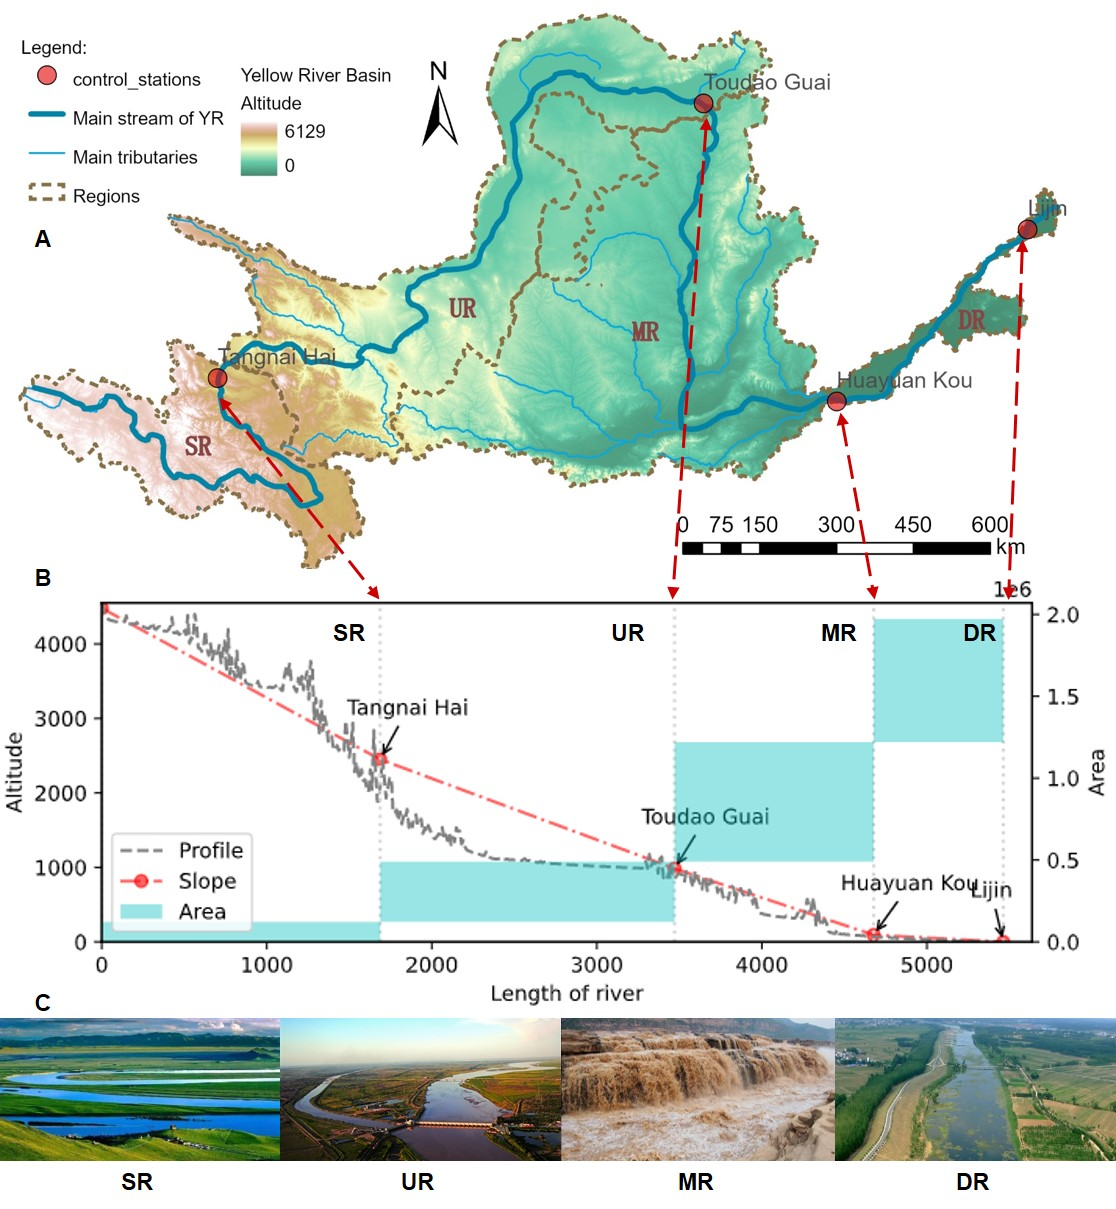
\includegraphics[width=0.6\textwidth]{sup/s1_study_area.jpg}
    \caption{
        The study area.
        \textbf{A.} Diagram of the YRB and the subdivision of the basin (SR: Source Region, UR: Upper Region, MR: Middle Region, DR: Downstream region).
        \textbf{B.} Profile of the main channel of the Yellow River. The hydrological stations control the SR, UR, MR and DR.
        \textbf{C.} Typical landscapes in different regions in the YRB.
    }
    \label{fig:YRB}
\end{figure*}

% % 补充图片4:天然水资源量
% \begin{figure*}[tb]
%     \centering
%     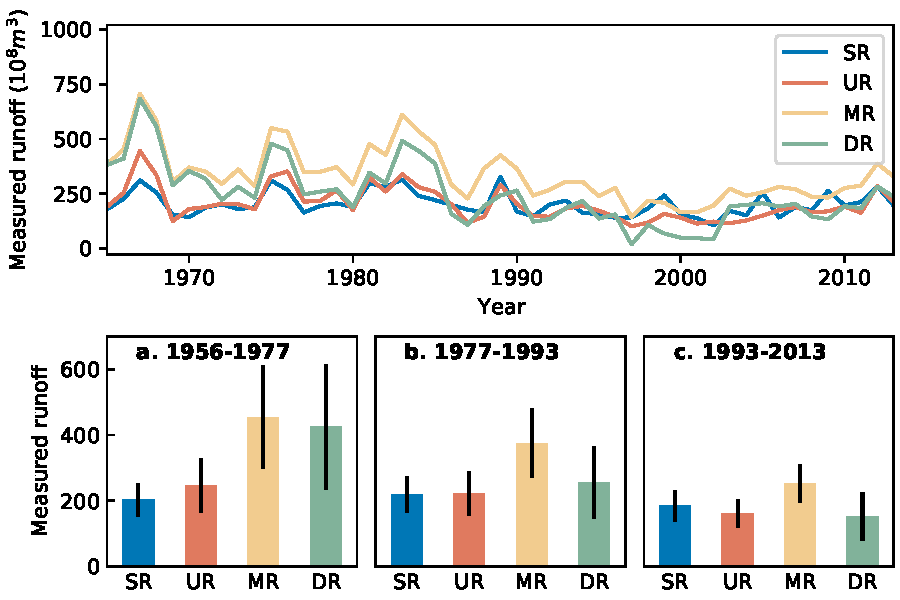
\includegraphics[width=0.8\textwidth]{sup/sf_measured_runoff.pdf}
%     \caption{Water resources in different regions.
%         \textbf{A,} changing trend of measured runoff,
%         \textbf{B, C and D} average measured runoff within different periods.
%         \textbf{E, F and G} average total water consumptions within different periods.
%     }
%     \label{fig:water resources}
% \end{figure*}
